%%%%%%%%%%%%%%%%%%%%%%%%%%%%%%%%%%%%%%%%%
% Short Sectioned Assignment
% LaTeX Template
% Version 1.0 (5/5/12)
%
% This template has been downloaded from:
% http://www.LaTeXTemplates.com
%
% Original author:
% Frits Wenneker (http://www.howtotex.com)
%
% License:
% CC BY-NC-SA 3.0 (http://creativecommons.org/licenses/by-nc-sa/3.0/)
%
%%%%%%%%%%%%%%%%%%%%%%%%%%%%%%%%%%%%%%%%%

%----------------------------------------------------------------------------------------
%	PACKAGES AND OTHER DOCUMENT CONFIGURATIONS
%----------------------------------------------------------------------------------------

\documentclass[paper=a4, fontsize=11pt]{scrartcl} % A4 paper and 11pt font size

\usepackage[T1]{fontenc} % Use 8-bit encoding that has 256 glyphs
\usepackage{fourier} % Use the Adobe Utopia font for the document - comment this line to return to the LaTeX default
\usepackage[english]{babel} % English language/hyphenation
\usepackage{amsmath,amsfonts,amsthm} % Math packages
\usepackage[utf8]{inputenc}
\usepackage{graphicx}
\usepackage{tabularx}
\usepackage{longtable}
\usepackage{threeparttable}
\usepackage{booktabs}
\usepackage{listings}
\usepackage[numbered,autolinebreaks,useliterate]{mcode}
\usepackage{float}
\usepackage{algpseudocode}

\usepackage{lipsum} % Used for inserting dummy 'Lorem ipsum' text into the template

\usepackage{sectsty} % Allows customizing section commands
\allsectionsfont{\centering \normalfont\scshape} % Make all sections centered, the default font and small caps

\usepackage{fancyhdr} % Custom headers and footers
\pagestyle{fancyplain} % Makes all pages in the document conform to the custom headers and footers
\fancyhead{} % No page header - if you want one, create it in the same way as the footers below
\fancyfoot[L]{} % Empty left footer
\fancyfoot[C]{} % Empty center footer
\fancyfoot[R]{\thepage} % Page numbering for right footer
\renewcommand{\headrulewidth}{0pt} % Remove header underlines
\renewcommand{\footrulewidth}{0pt} % Remove footer underlines
\setlength{\headheight}{13.6pt} % Customize the height of the header

\numberwithin{equation}{section} % Number equations within sections (i.e. 1.1, 1.2, 2.1, 2.2 instead of 1, 2, 3, 4)
\numberwithin{figure}{section} % Number figures within sections (i.e. 1.1, 1.2, 2.1, 2.2 instead of 1, 2, 3, 4)
\numberwithin{table}{section} % Number tables within sections (i.e. 1.1, 1.2, 2.1, 2.2 instead of 1, 2, 3, 4)

\setlength\parindent{0pt} % Removes all indentation from paragraphs - comment this line for an assignment with lots of text

% new command for short vertical space
\newcommand{\vertbreak}{\vspace{1.75 mm}}

% define "struts", as suggested by Claudio Beccari in
%    a piece in TeX and TUG News, Vol. 2, 1993.
\newcommand\Tstrut{\rule{0pt}{2.6ex}}         % = `top' strut
\newcommand\Bstrut{\rule[-0.9ex]{0pt}{0pt}}   % = `bottom' strut

%----------------------------------------------------------------------------------------
%	TITLE SECTION
%----------------------------------------------------------------------------------------

\newcommand{\horrule}[1]{\rule{\linewidth}{#1}} % Create horizontal rule command with 1 argument of height

\title{	
\normalfont \normalsize 
\textsc{Faculdade de Engenharia da Universidade do Porto} \\ [25pt] % Your university, school and/or department name(s)
\horrule{0.5pt} \\[0.4cm] % Thin top horizontal rule
\LARGE Machnine Learning (PDEEC0049 : 15-782PP)\\ \Large Homework 2 \\ % The assignment title
\horrule{2pt} \\[0.5cm] % Thick bottom horizontal rule
}

\author{António Damião das Neves Rodrigues (200400437 : 700098386)} % Your name

\date{\normalsize\today} % Today's date or a custom date

\begin{document}

\maketitle % Print the title

\section{Problem 1}

Let us consider the losses one gets for wrongly choosing $Y_i = 0$ and 
$Y_i = 1$, for now disregarding the reject option and its loss value 
$\lambda$. One can define a loss matrix \textbf{L} for such problem as 
follows:

\begin{equation}
\begin{split}
    \textbf{L}  &= \begin{bmatrix} \ell_{00} & \ell_{01} \\ \ell_{10} & \ell_{11} \end{bmatrix} = \begin{bmatrix} 0 & 1 \\ 1 & 0 \end{bmatrix}
    \label{eq:1-loss-matrix}
\end{split}
\end{equation}

In~\ref{eq:1-loss-matrix}, $\ell_{01}$ represents the cost for deciding for $Y_i = 1$ 
when the right choice would be $Y_i = 0$. The costs for deciding for $Y_i = 0$ 
and $Y_i = 1$ would then be given by the following expressions:

\begin{equation}
\begin{split}
    \mathcal{L}(Y_i = 0)    &= \ell_{00}P(Y_i = 0|x_i) + \ell_{10}P(Y_i = 1|x_i)\\
                            &= 0 \times (1 - p_i) + 1 \times p_i\\
                            &= p_i\\
    \mathcal{L}(Y_i = 1)    &= \ell_{01}P(Y_i = 0|x_i) + \ell_{11}P(Y_i = 1|x_i)\\
                            &= 1 \times (1 - p_i) + 0 \times p_i\\
                            &= (1 - p_i)
    \label{eq:1-losses}
\end{split}
\end{equation}

Taking a reject option into consideration, one would decide for it when such a 
choice would be advantageous relative to choosing $Y_i = 0$ and 
$Y_i = 1$. Since we are given a quantifiable cost for choosing the 
reject option, $\lambda$, one should choose it when 
$\mathcal{L}(Y_i = 0) > \lambda \wedge \mathcal{L}(Y_i = 1) > \lambda$, or 
$p_i > \lambda \wedge 1 - p_i > \lambda$. This reasoning results in the optimal 
decision rule given in~\ref{eq:1-final}.

\begin{equation}
    \text{choose} \left\{ 
        \begin{array}{rl}
            Y_i = 0, &\mbox{ \text{if $p_i < \frac{1}{2} \wedge p_i < \lambda$}} \\
            Y_i = 1, &\mbox{ \text{if $\frac{1}{2} < p_i \wedge 1 - \lambda < p_i$}} \\
            \text{reject}, &\mbox{ \text{if $ \lambda < p_i < 1 - \lambda$}}
        \end{array} \right.
    \label{eq:1-final}
\end{equation}

\section{Problem 2}

\subsection{}
\label{subsec:2-1}

Our objective is to determine the posterior probabilities $P(C_k|F_1,F_2,F_3,F_4)$, 
using Bayes' Theorem in the form shown in expression~\ref{eq:2-1:bayes}:

\begin{equation}
\begin{split}
    P(C_k|F_1,F_2, ...,F_n)  &= \frac{P(F_1,F_2, ...,F_n|C_k)P(C_k)}{P(F_1,F_2, ...,F_n)}
    \label{eq:2-1:bayes}
\end{split}
\end{equation}

In this case, we cannot use the naive Bayes assumption. This assumption 
treats $F_1, F_2, ..., F_n$ as conditionally independent (given the class $C_k$) 
between each other, which would allow us to easily compute the factor 
$P(F_1,F_2,F_3,F_4|C_k)$ as $\prod_{i=1}^{4} P(F_i|C_k)$. In this case we would 
only have to model five parameters, each of the class-conditional probabilities 
$P(F_i|C_k)$ and a prior $P(C_1)$ (since $k = 2$, $P(C_2)$ would follow as 
$1 - P(C_1)$). In general, using the naive Bayes assumption, we have to model 
$k \times n + (k - 1)$ parameters. The problem would be solved as proposed in 
problem 2.2 (see Section~\ref{subsec:2-2}).\\

Without the naive Bayes assumption, we would have to compute the factor 
$P(F_1,F_2,F_3,F_4|C_k)$ in a different way, since features 
$F_1, F_2, ..., F_n$ are no longer treated as conditionally independent between 
each other.\\ 

Using the product rule of probability, the expression 
$P(F_1, ..,F_n|C_k)$ is equivalent to $\frac{P(C_k,F_1, ..,F_n)}{C_k}$. 
The numerator is the joint probability distribution of $C_k, F_1, ..,F_n$. This 
can be represented by the chain rule of probability, as given in 
expression~\ref{eq:2-1-chain}, for $C_k, F_1, F_2, ..., F_n$:

\begin{equation}
\begin{split}
    P(C_k, F_1,F_2, ...,F_n) &= P(C_k)P(F_1|C_k)P(F_2|F_1,C_k) ... P(F_n|F_{n-1}, ..., C_k)
    \label{eq:2-1-chain}
\end{split}
\end{equation}

One should note that the dependence of each feature $F_i$ on other features 
$F_j$ now ask for the determination of much more parameters than for the 
naive Bayes case. E.g. for $P(F_2|F_1,C_k)$, we must execute a sum 
for each of the 5 values the feature $F_1$ can take, i.e.:

\[P(F_2|F_1,C_k) = \sum_{i=1}^{5} P(F_2|F_1 = q_i,C_k)\]

This particular example requires the calculation of 5 parameters 
$P(F_2|F_1 = q_i,C_k)$, for a given $C_k$. For conditional probability factors 
that depend on multiple features, one must account for the combinations of 
values $q$ between features $F_i$ and $F_j$. Generalizing, the total number of 
class-conditional parameters to determine for our case with 4 features which can assume 
5 values is $5^3 + 5^2 + 5^1 + 1 = 5^4 - 1$. Considering the 2 classes $C_1$ and 
$C_2$, the number becomes $2(5^4 - 1)$.\\

In order to train the classifier, one would arrange the 
training data in a suitable table fashion, determine the relative frequencies 
for each one of these class-conditional parameters (plus the priors) and then 
determine the expressions for the posteriors $P(C_k|F_1,...,F_n)$.\\

\subsection{}
\label{subsec:2-2}

First, let us consider the following:

\begin{itemize}

    \item A binary class $Y$, which can take values $y \in \{0,1\}$. A value 
            $y = 0$ means a phone didn't last one year, while $y = 1$ means 
            a phone lasted one year.
    \item $G$ a feature assuming values $g \in \{0,1\}$. It is used to 
            indicate if the user gender is female (0) or male (1).
    \item $C$ a feature assuming values $c \in \{0,1\}$. It is used to 
            indicate if the phone's colors is 
            black (0) or white (1).
    \item $T$ a feature assuming values $t \in \{0,1\}$. It is used to 
            indicate if the phone's type is 
            keypad-based (0) or touchscreen-based (1).

\end{itemize}

The problem asks us to compare $P(Y = 1|G = 1, C = 1,T = 1)$ and 
$P(Y = 0|G = 1, C = 1,T = 1)$. To compute these two values, we can use Bayes 
Theorem in the form given in~\ref{eq:2-2-mult-feat} to calculate these as 
posterior probabilities.

\begin{equation}
\begin{split}
    P(Y = y|G = g, C = c, T = t)  &= \frac{P(G = g, C = c, T = t|Y = y)P(Y = y)}{P(G = g, C = c, T = t)}
    \label{eq:2-2-mult-feat}
\end{split}
\end{equation}

For simplicity, we will assume that features $G$, $C$ and $T$ are 
conditionally independent (i.e. given $Y = y$) between each other, making 
$P(G = g, C = c,T = t|Y = y) = P(G = g|Y = y)P(C = c|Y = y)P(T = t|Y = y)$, 
i.e. we will be making the naive Bayes assumption.\\ 

Before applying Bayes theorem, we must compute the relevant 
values of the class conditional probabilities and the priors. These can be 
obtained by working out the relative frequencies among 
the data given in the exercise.\\ 

E.g. in order to find the value for 
$P(G = 1|Y = 1)$, count the number of `Male' cases which `lasted for more than a 
year', $k$, and divide this number by the total amount of cases which lasted 
for more than a year, $\ell$, resulting in  resulting in $P(G = 1|Y = 1) = \frac{k}{\ell} 
= \frac{3}{5}$.\\ 

The values 
in Tables~\ref{tab:2-class-conditional} and~\ref{tab:2-priors} show the values 
of the class-conditional and prior probabilities for the problem in question, 
by application of the previously described process.\\

\begin{table}[h!]
\begin{center}
        \begin{tabularx}{0.3125\textwidth}{ c | c | c  }
            %\hline
                        & Y = 1 & Y = 0 \\ [0.5ex]
            \hline 
            $P(G = 1|Y)$    & $\frac{3}{5}$ \Tstrut     & $\frac{2}{5}$ \Tstrut   \\ [1.5ex]
            $P(C = 1|Y)$    & $\frac{1}{5}$      & $\frac{3}{5}$    \\ [1.5ex]
            $P(T = 1|Y)$    & $\frac{2}{5}$      & $\frac{3}{5}$    \\ [1.5ex]
            %\hline
        \end{tabularx}

    \caption{Class-conditional probabilities for Problem 2.2.}
    \label{tab:2-class-conditional}
    \end{center}
\end{table}

\begin{table}[h!]
\begin{center}
        \begin{tabularx}{0.25\textwidth}{ c | c | c  }
            %\hline
                        & Y = 1 & Y = 0 \\ [0.5ex]
            \hline 
            $P(Y)$    & $\frac{5}{10}$ \Tstrut     & $\frac{5}{10}$ \Tstrut   \\ [1.5ex]
            %\hline
        \end{tabularx}

    \caption{Prior probabilities for Problem 2.2.}
    \label{tab:2-priors}
    \end{center}
\end{table}

With the class-conditional and prior probability values, one can now apply 
Bayes' theorem to calculate the posteriors $P(Y = 1|G = 1, C = 1,T = 1)$ and 
$P(Y = 0|G = 1, C = 1,T = 1)$ and compare their values:

\begin{equation}
\begin{split}
    P(Y = 1|M,W,T)  &= \frac{P(G = 1|Y = 1)P(C = 1|Y = 1)P(T = 1|Y = 1)P(Y = 1)}{P(G = 1, C = 1,T = 1)}\\
                    &= \frac{\frac{3 \times 1 \times 2}{125} \times \frac{1}{2}}{P(G = 1, C = 1,T = 1)} = \frac{\frac{6}{250}}{P(G = 1, C = 1,T = 1)}\\     
\\
    P(Y = 0|M,W,T)  &= \frac{P(G = 1|Y = 0)P(C = 1|Y = 0)P(T = 1|Y = 0)P(Y = 0)}{P(G = 1, C = 1,T = 1)}\\
                    &= \frac{\frac{2 \times 3 \times 3}{125} \times \frac{1}{2}}{P(G = 1, C = 1,T = 1)} = \frac{\frac{18}{250}}{P(G = 1, C = 1,T = 1)}
    \label{eq:2-2-posteriors}
\end{split}
\end{equation}

Since the factor on the denominator is common to both posterior values, one 
must only evaluate the numerator to verify which one is larger. In this case, 
$P(Y = 1|G = 1, C = 1, T = 1) < P(Y = 0|G = 1, C = 1, T = 1)$. Therefore, a 
white colored phone with touchscreen in the hands of a male individual is less 
likely to last for more than one year than not.

\section{Problem 3}

The conventions and notation specified on slide 2 
in~\cite{Cardoso2013} will be used throughout sections 3.1 to 3.3.

\subsection{}
\label{subsec:3-1}

\begin{lstlisting}[label=lst:regression,caption={MATLAB function for calculating 
the coefficients of the linear regression on a given training dataset, 
composed by the arrays.}]
function [weights] = regression(train_data_X, train_data_Y)
%% number rows in train_data_X = number of examples
%% number columns in train_data_X = dimension
%% train_data_Y

weights = (train_data_X'*train_data_X)\(train_data_X'*train_data_Y);

return;

\end{lstlisting}

The code on Listing~\ref{lst:regression} was obtained by deducing the normal equation 
of the error function~\ref{eq:3-1-non-regular-error}, in matrix notation, leading 
to the expression shown in~\ref{eq:3-1-non-regular-normal}.\vertbreak

\begin{equation}
    \mathcal{L}(\textbf{w},S) = \frac{1}{2}\sum_{n=0}^{N}(y_n - \textbf{w}^{t}\textbf{x}_n)^{2}
    \label{eq:3-1-non-regular-error}
\end{equation}

\begin{equation}
\begin{split}
    \textbf{X}^{t}\textbf{X}\textbf{w} &= \textbf{X}^{t}\textbf{y}\\
    \textbf{w} &= \left(\textbf{X}^{t}\textbf{X}\right)^{-1}\textbf{X}^{t}\textbf{y}
    \label{eq:3-1-non-regular-normal}
\end{split}
\end{equation}

Figure~\ref{fig:3-1} was obtained by setting the 4\textsuperscript{th} argument 
of the function \verb?poly_regression()? to \textbf{9} (i.e. in order to obtain 
the polynomial regression of degree 9 on the dataset composed by 
\verb?train_data_X? and \verb?train_data_Y?), on the MATLAB 
file \verb?testRegression.m?.

\begin{figure}[H]

    \centering
    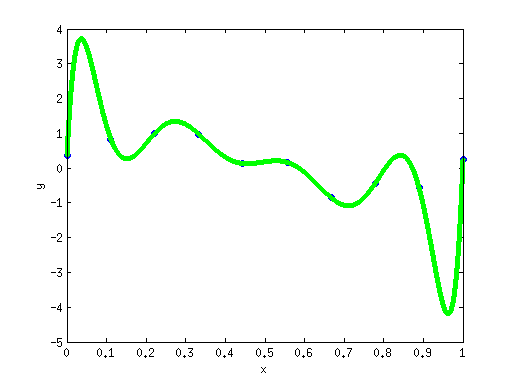
\includegraphics[width=0.85\textwidth]{figures/3-1.png}
    \caption{Plot of the polynomial function $\sum_{n=0}^{9} w_n x^{n}$, over values of $x$ in the 
            interval $[0,1]$  using the coeficients $w_n$ produced by the code 
            shown in Listing~\ref{lst:regression}.}
    \label{fig:3-1}

\end{figure}

\subsection{}
\label{subsec:3-2}

\begin{equation}
    \mathcal{L}(\textbf{w},S) = \frac{1}{2}\sum_{n=0}^{N}c_n(y_n - \textbf{w}^{t}\textbf{x}_n)^{2} + \frac{1}{2}\lambda\textbf{w}^{t}\textbf{w}
    \label{eq:3-1-regular-error}
\end{equation}

In matrix notation, \ref{eq:3-1-regular-error} becomes:

\begin{equation}
\begin{split}
    \mathcal{L}(\textbf{w},S) &= \frac{1}{2}\left[\left(\textbf{X}\textbf{w} - \textbf{y}\right)^{t}\textbf{C}\left(\textbf{X}\textbf{w} - \textbf{y}\right) + \lambda\textbf{w}^{t}\textbf{w}\right]\\
    &= \frac{1}{2}\left[\left(\textbf{w}^{t}\textbf{X}^{t} - \textbf{y}^{t}\right)\left(\textbf{C}\textbf{X}\textbf{w} - \textbf{C}\textbf{y}\right) + \lambda\textbf{w}^{t}\textbf{w}\right]\\
    &= \frac{1}{2}\left[\textbf{w}^{t}\textbf{X}^{t}\textbf{C}\textbf{X}\textbf{w} - \textbf{w}^{t}\textbf{X}^{t}\textbf{C}\textbf{y} - 
\textbf{y}^{t}\textbf{C}\textbf{X}\textbf{w} - \textbf{y}^{t}\textbf{C}\textbf{y} + \lambda\textbf{w}^{t}\textbf{w}\right]\\
    \\
    \text{with} \quad \textbf{C} &= \begin{bmatrix} c_1 & 0 & 0 & ... & 0 \\ 0 & c_2 & 0 & ... & 0 \\ 0 & 0 & c_3 & ... & 0 \\ ... & ... & ... & ... & ... \\ 0 & 0 & 0 & ... & c_n \end{bmatrix}
    \label{eq:3-2-regular-matrix}
\end{split}
\end{equation}

To obtain the normal equations, take the derivative and set to zero, as in 
expression~\ref{eq:3-2-regular-matrix-normal}:

\begin{equation}
\begin{split}
    0 &= \frac{\partial \mathcal{L}}{\partial \textbf{w}}\\
    0 &= \frac{1}{2}\left[\frac{\partial}{\partial \textbf{w}}\left(\textbf{w}^{t}\textbf{X}^{t}\textbf{C}\textbf{X}\textbf{w}\right) 
        - \frac{\partial}{\partial \textbf{w}}\left(\textbf{w}^{t}\textbf{X}^{t}\textbf{C}\textbf{y}\right) 
        - \frac{\partial}{\partial \textbf{w}}\left(\textbf{y}^{t}\textbf{C}\textbf{X}\textbf{w}\right) 
        - \frac{\partial}{\partial \textbf{w}}\left(\textbf{y}^{t}\textbf{C}\textbf{y}\right) 
        + \lambda\frac{\partial}{\partial \textbf{w}}\left(\textbf{w}^{t}\textbf{w}\right)\right]\\
    0 &= \frac{1}{2}\left[
        \left(\left(\textbf{X}^{t}\textbf{C}\textbf{X}\right)^{t} + \left(\textbf{X}^{t}\textbf{C}\textbf{X}\right)\right)\textbf{w} 
        - \textbf{X}^{t}\textbf{C}\textbf{y} 
        - \left(\textbf{y}^{t}\textbf{C}\textbf{X}\right)^{t} 
        - 0 
        + 2\lambda\textbf{w}\right]\\
    0 &= \frac{1}{2}\left[
        2\left(\textbf{X}^{t}\textbf{C}\textbf{X}\right)\textbf{w} 
        - 2\textbf{X}^{t}\textbf{C}\textbf{y} 
        + 2\lambda\textbf{w}\right]\\
    0 &= \left(\textbf{X}^{t}\textbf{C}\textbf{X}\right)\textbf{w} 
        - \textbf{X}^{t}\textbf{C}\textbf{y} 
        + \lambda\textbf{w}\\
    \textbf{X}^{t}\textbf{C}\textbf{y} &= \left(\textbf{X}^{t}\textbf{C}\textbf{X} + \lambda\textbf{I}\right)\textbf{w} 
    \label{eq:3-2-regular-matrix-normal}
\end{split}
\end{equation}

\subsection{}
\label{subsec:3-3}

\begin{lstlisting}[label=lst:reg-regression,caption={MATLAB function for 
calculating the coefficients of the linear regression on a given training 
dataset, including a regularization factor.}]
function [weights] = regularizedregression(train_data_X, train_data_Y, c, lambda)
%% number rows in train_data_X = number of examples
%% number columns in train_data_X = dimension

% diagonal matrix C built as 
% [c1 0 0 ... 0 ; 0 c2 0 ... 0 ; ... ; 0 0 0 ... cn] 
C = diag(c);

% dimension for the identity matrix to be scaled by the lambda 
% (regularization) factor
D = size(train_data_X,2);

weights = ((train_data_X'*C*train_data_X) + lambda*eye(D))\(train_data_X'*C*train_data_Y);

return;
\end{lstlisting}

The code on Listing~\ref{lst:reg-regression} was obtained by implementing 
expression~\ref{eq:3-2-regular-matrix-normal} in MATLAB, in order to 
\textbf{w}. The vector \verb?c?, passed to the function 
\verb?regularizedregression()? as a $1 \times N$ vector, $N$ being the number 
of lines in \textbf{X} (i.e. the number of samples in the dataset from PRMLBishop~\cite{Bishop2006}), 
holds the coefficients $c_n$ shown in expression~\ref{eq:3-1-regular-error}. The 
expression in line 7 of Listing~\ref{lst:reg-regression} diagonalizes the 
vector \verb?c? into a $N \times N$ matrix \textbf{C}, which holds the 
coefficients $c_n$ as defined in 
expression~\ref{eq:3-2-regular-matrix}.\vertbreak

\begin{figure}[H]

    \centering
    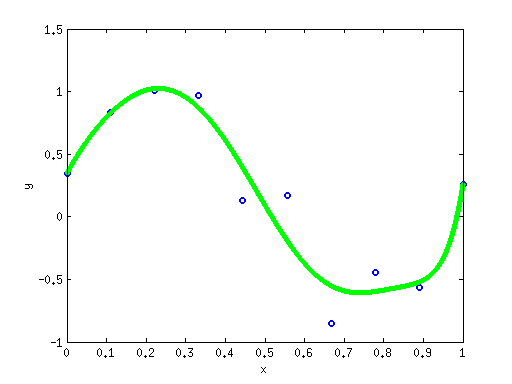
\includegraphics[width=0.85\textwidth]{figures/3-3.png}
    \caption{Plot of the polynomial function $\sum_{n=0}^{9} w_n x^{n}$, over 
            values of $x$ in the interval $[0,1]$  using the coefficients $w_n$ 
            produced by regularized regression 
            expression~\ref{eq:3-2-regular-matrix-normal} and the code 
            shown in Listing~\ref{lst:reg-regression}. Regularization 
            factor $\lambda = e^{-18}$.}
    \label{fig:3-3}

\end{figure}

Figure~\ref{fig:3-3} was obtained by setting the 4\textsuperscript{th} argument 
of the function \verb?poly_regression()? to 9 (i.e. in order to obtain 
the polynomial regression of degree 9 on the dataset composed by 
\verb?train_data_X? and \verb?train_data_Y?), on the MATLAB 
file \verb?testRegression.m?. Of course, the value of the \verb?weights? 
variable in the MATLAB file \verb?poly_regression.m? is set by the function 
\verb?regularizedregression()?, with \verb?lambda? $= e^{-18}$.\\

\bibliographystyle{plain}
\bibliography{hw2.bib}

\end{document}
